%% litdiscover.tex — Annotation draft for PI review
%% Compile: pdflatex litdiscover && bibtex litdiscover && pdflatex litdiscover && pdflatex litdiscover
% \documentclass[12pt,a4paper]{article}
\documentclass[conference]{IEEEtran}

% \usepackage[margin=1.25in, top=1in, bottom=1in]{geometry}
\usepackage[utf8]{inputenc}
\usepackage[T1]{fontenc}
\usepackage{lmodern}
\usepackage{microtype}
% \usepackage{parskip}
% \usepackage{setspace}
% \usepackage{titlesec}
\usepackage{hyperref}
\usepackage{url}
\usepackage{graphicx}
\usepackage{booktabs}
\usepackage{array}
\usepackage{tabularx}
\usepackage{caption}
\usepackage{subcaption}
\usepackage{xcolor}
\usepackage{soul}         % for \hl{} yellow highlight
\usepackage{mdframed}
\usepackage{amsmath}
\usepackage[numbers]{natbib}

% ── Colours ──────────────────────────────────────────────────────────────────
\definecolor{litblue}{RGB}{33,102,172}
\definecolor{missingcite}{RGB}{220,50,47}

% ── Hyperref setup ────────────────────────────────────────────────────────────
\hypersetup{
  colorlinks=true,
  linkcolor=litblue,
  citecolor=litblue,
  urlcolor=litblue,
  pdftitle={Robust Literature Discovery from Minimal Seeds},
  pdfauthor={},
}

% ── Figure path ───────────────────────────────────────────────────────────────
\graphicspath{{../data-aps/outputs/pub_figures/}}

% ── Convenience macros ────────────────────────────────────────────────────────
\newcommand{\ldiscover}{\textsc{LitDiscover}}
\newcommand{\todo}[1]{\textcolor{missingcite}{\textbf{[#1]}}}
\newcommand{\cn}{\todo{CITATION NEEDED}}   % missing citation marker

% ─────────────────────────────────────────────────────────────────────────────
\title{Robust Literature Discovery from Minimal Seeds:\\
  Validating \ldiscover{} on APS Citation Benchmarks and Live Surveys}

\author{%
  \IEEEauthorblockN{David Goh}
  \IEEEauthorblockA{Department of Computer Science\\University of Toronto\\daveed@cs.toronto.edu}
  \and
  \IEEEauthorblockN{Xiaobai Sun}
  \IEEEauthorblockA{Department of Computer Science\\Duke University\\xiaobai@cs.duke.edu}
}

\begin{document}

\maketitle

% ─────────────────────────────────────────────────────────────────────────────
\begin{abstract}
Automated literature discovery must do something retrieval cannot: recover a topic's
literature from almost nothing. We introduce \ldiscover{}, a queue-driven engine
that navigates citation graphs through three coordinated mechanisms --- bidirectional
traversal, Pareto-filtered hub suppression, and yield-gated continuation. Using the
American Physical Society (APS) 2022 dataset (709,803 papers, 9,833,191 edges) as a
closed benchmark, we evaluate recovery from minimal seed sets ($k \in \{1,2,3,4,5,10\}$)
against three landmark survey papers. \ldiscover{} achieves near-complete bibliography
recovery from as few as one to five seeds, demonstrating that high-recall discovery is
achievable under realistic minimal-seeding conditions. Residual misses are structurally
peripheral --- low in-degree papers that are adjacent to but below the traversal's
productive horizon --- not randomly distributed across the domain. Live validation on three
open-domain surveys confirms that the same yield-governed control logic transfers outside
the benchmark: yield collapse is a reliable operational signal that engages at a principled
structural boundary, with domain density governing how far the coverage frontier extends.
\end{abstract}

% ─────────────────────────────────────────────────────────────────────────────
\section{Introduction}

The central practical problem in automated literature review is not merely how to summarize
papers once they have been found, but how to \textbf{discover} a topic comprehensively from
incomplete starting information. Real users rarely begin with a complete domain map or even
a strong initial bibliography. More commonly, they begin with a query, a few candidate
papers, and an uncertain boundary between relevant and irrelevant work. A useful review
system must therefore solve a discovery problem under sparse initial supervision.

Citation graphs provide a natural substrate for this task because they expose relational
structure that keyword search alone cannot recover \citep{Redner2005}. A paper's references
reveal backward intellectual lineage, while incoming citations reveal later work that builds
on or reacts to it. In principle, repeated traversal over this graph should allow a system
to expand from a small local starting point into a much larger topical neighbourhood. In
practice, however, naive traversal fails because citation networks are highly asymmetric
\citep{Barabasi2016, BarabasiAlbert1999}. Backward traversal is naturally bounded by
bibliography length, whereas forward traversal rapidly encounters generic high-degree hubs
that connect many otherwise distant parts of the literature. Unconstrained exploration
therefore turns a promising discovery process into an intractable screening problem.

\ldiscover{} addresses this problem as a bounded traversal architecture. Rather
than treating literature discovery as open-ended graph expansion, it organises discovery
around a queue-driven loop in which search, screening, traversal, and escape operations
are all subordinated to a single yield-governed control policy. Three architectural ideas
are central. First, the system uses \textbf{bidirectional traversal}, because neither
backward nor forward expansion alone is sufficient to recover a topic. Second, it applies
\textbf{Pareto-filtered forward expansion} to suppress high-degree hubs that
disproportionately drive graph explosion and topic drift. Third, it uses a
\textbf{yield-gated continuation rule} to determine when local expansion remains productive
and when the system should instead jump to a fresh part of the graph.

This paper evaluates \ldiscover{} in the regime that matters most for deployment:
\textbf{minimal seeding} ($k \in \{1,2,3,4,5,10\}$). The evaluation uses APS as a closed
citation universe and derives gold sets directly from published survey bibliographies, giving
a precise and bias-free recall metric. The same configuration is then run against three live
open-domain surveys via the Semantic Scholar API, testing whether the yield-governed control
logic transfers outside the benchmark.

The paper makes four contributions. First, it gives a structural account of why bounded
traversal is necessary: hub suppression and yield stopping are principled responses to
power-law degree skew, not arbitrary heuristics. Second, it shows that \ldiscover{} achieves
near-complete recall from as few as one to five seed papers --- the regime real users actually
occupy. Third, it characterises the residual gap through miss analysis, showing that what the
system misses is structurally peripheral rather than randomly lost; this matters because it
distinguishes a principled stopping boundary from architectural failure, and informs when
relaxing the Pareto or yield parameters would actually help. Fourth, it confirms via live
validation that yield collapse is an operational signal in deployment, not just an offline
metric; this is non-trivial because the closed-corpus simulation cannot demonstrate that the
stopping rule generalises to open citation graphs with incomplete indexing and temporal gaps.

% ─────────────────────────────────────────────────────────────────────────────
\section{Related Work}

This paper sits at the intersection of three areas.

\textbf{Citation-graph analysis} has characterised degree distributions, clustering, and
community structure in academic networks \citep{BarabasiAlbert1999, Price1965}. Heavy-tailed
in-degree is well documented \citep{Redner2005, Barabasi2016}: a small fraction of papers
mediate a disproportionate share of cross-domain connectivity, motivating the Pareto filter
design. Recent LLM-based simulation
work corroborates this mechanistically --- \citet{Ji2025CiteAgent} find that the
recommendation algorithm's tendency to surface highly cited papers is a stronger driver of
preferential attachment than author citation bias, explaining how hubs self-reinforce over time.

\textbf{Automated systematic review and evidence synthesis} spans a spectrum from
manual-heavy to fully automated. Early tools such as SWIFT-Review \citep{Howard2016} and
RobotSearch \citep{Marshall2019} combine keyword or ML-based screening with manual corpus
assembly. Active-learning frameworks such as ASReview \citep{vandeSchoot2021} go further
by prioritising which pre-assembled candidates to screen first, substantially reducing manual
effort --- but all of these assume the candidate pool is already given. LLM-assisted
exploration tools (Elicit~\citep{Elicit2024}, ResearchRabbit~\citep{ResearchRabbit2025})
extend this with query-driven discovery, but without a formal stopping criterion. \ldiscover{}
sits at the missing end of this spectrum: it \textit{constructs} the candidate pool via graph
traversal before screening begins, governed by an explicit yield-based termination rule.

\textbf{Graph compression and hub-aware sampling} provides the theoretical grounding for the
Pareto filter. Work on $k$-core decomposition \citep{Batagelj2003} and degree-constrained
sampling \citep{Stumpf2005} shows that removing high-degree hubs substantially reduces edge
volume while preserving reachability. The Pareto filter is a soft variant of this idea applied
to the forward traversal frontier.

These three areas converge in a way that directly motivates \ldiscover{}. Citation-graph
analysis supplies the observation that degree skew is structural and predictable ---
it is not a nuisance to be filtered out after the fact, but a property that should
govern traversal design from the outset. Systematic review methodology supplies the
recall objective: what matters is not sampling the literature but recovering it
completely enough to support synthesis. Hub-aware sampling supplies the filter
mechanism: the Pareto threshold is a soft analogue of core decomposition, applied
not to compress a static graph but to constrain a live traversal frontier. No prior
tool connects all three: snowballing tools lack principled stopping; systematic
review tools assume a pre-assembled corpus; graph compression work does not address
the cold-start or recall-framing concerns of literature discovery.

\ldiscover{} formalises and automates the snowballing methodology \citep{Wohlin2014} ---
systematic bidirectional citation chaining from seed papers --- replacing manual curation
with a yield-governed queue and LLM screening. The distinguishing feature relative to prior
citation-expansion tools (CiteSpace~\citep{Chen2006}, Connected Papers~\citep{ConnectedPapers})
is the minimal-seed framing: those systems assume a large anchor set; \ldiscover{} bootstraps
a domain bibliography from two to five entry points.

% ─────────────────────────────────────────────────────────────────────────────
\section{Architecture and Control Logic}

\ldiscover{} is best understood as a queue-driven discovery loop rather than a static
retrieval pipeline. At a high level, the system alternates between \textbf{search},
\textbf{screening}, \textbf{traversal}, and \textbf{escape} operations until it reaches
a stable state. The logic can be summarised as:

\begin{center}
\texttt{SEED → SEARCH → SCREEN → TRAVERSE → ESCAPE → STABLE}
\end{center}

The system begins from an initial seed set, which may consist of search results,
user-supplied papers, or a mixture of the two. These papers enter a unified screening
queue. Screening decisions then identify which items should be retained as relevant and
therefore eligible for expansion. Expansion occurs through citation traversal, but only
under bounded conditions.

The first architectural principle is \textbf{bidirectional traversal}. Backward traversal
follows references made by included papers and is essential because relevant older work is
often directly cited by on-topic seeds. Forward traversal follows papers that cite included
items and is equally important because it exposes later developments that no initial
bibliography can contain. Yet forward traversal is also the primary source of explosion.
Foundational papers, methods papers, and generic benchmark papers accumulate citations
across many subfields, so blindly following their incoming edges pushes the system into
large off-topic regions of the graph.

The second architectural principle is therefore \textbf{Pareto-filtered forward expansion}.
Rather than expanding equally through all forward neighbours, \ldiscover{} suppresses a
high-degree tail of forward candidates. The rationale is graph-theoretic: in a heavy-tailed
network \citep{Barabasi2016}, a relatively small fraction of nodes mediate a disproportionate
share of edges. Those nodes are often precisely the hubs that maximise breadth while minimising
topical specificity. The Pareto filter is thus not only an efficiency device but also a
topicality control.

The third architectural principle is \textbf{yield-gated continuation}. Expansion is not
judged solely by how many new nodes it reaches, but by how many useful papers it produces
relative to the screening effort required. In the benchmark framing, this means that local
expansion should continue only when recent discoveries remain sufficiently fruitful; once
yield collapses, the system should either declare local exhaustion or invoke an
\textbf{Escape} step. Escape selects a new topical anchor from papers already recovered
but not yet used as traversal seeds --- in deployment, this is realised by a fresh keyword
query against an external index (Semantic Scholar); in the closed-corpus benchmark, it
selects from the accumulated recovered set. The selected anchor re-enters the traversal
loop as a new seed, bridging structurally disconnected or weakly connected clusters that
local expansion cannot reach.

This architecture formalises literature discovery as an alternating process of
\textbf{local exploitation} and \textbf{global re-entry}. Traversal explores dense
neighbourhoods already connected to the current frontier. The Escape step compensates for
structural gaps, indexing limitations, and disconnected subclusters by reintroducing a
search-based jump. The system therefore does not assume that a topic is perfectly recoverable
by graph traversal alone.

For the purposes of this paper, the key methodological claim is not only that final recall
is high, but that the \textbf{control mechanisms themselves work correctly}: yield collapse
reliably marks the boundary of productive local expansion, and the Escape step successfully
bridges disconnected clusters. Validating these behaviours --- measuring at what depth yield
collapses, whether Escape finds genuinely new territory, and whether the system terminates
without parameter sensitivity --- is as important as the aggregate recall figure, because it
establishes that the architecture is principled rather than tuned.

% ─────────────────────────────────────────────────────────────────────────────
\section{Closed-Corpus Benchmark and Experimental Design}

To evaluate the architecture under controlled conditions, we use the APS 2022 citation
dataset, a closed citation universe containing 709,803 papers and 9,833,191 citation edges
across American Physical Society journals \citep{APS2022}. The closed-corpus property is
essential because it ensures that every traversal step remains inside the benchmark, allowing
structural reachability, recall, and miss analysis to be defined precisely.

The ground-truth topical targets are derived from three highly cited survey papers published
in \textit{Reviews of Modern Physics} \citep{Imada1998,Bloch2008,Ozawa2019}. Each survey
contributes a bibliography that functions as a gold set for the associated topic.

\begin{table}[h]
\centering
\caption{APS benchmark surveys and gold sets.}
\label{tab:surveys}
\begin{tabular}{@{}llrr@{}}
\toprule
Survey ID & Topic & Year & Gold References \\
\midrule
\textbf{S1} & Metal-insulator transitions    & 1998 & 582 \\
\textbf{S2} & Ultracold gases                & 2008 & 432 \\
\textbf{S3} & Topological photonics          & 2019 & 387 \\
\bottomrule
\end{tabular}
\end{table}

The benchmark has two conceptual layers. The first is \textbf{structural motivation}, where
the survey papers are used to analyse citation-graph asymmetry and motivate bounded traversal.
The second is the \textbf{cold-start validation}, which simulates realistic user conditions
by replacing direct survey seeding with much smaller initial seed sets.

\begin{table}[h]
\centering
\caption{Experimental design for the cold-start validation.}
\label{tab:design}
\begin{tabular}{@{}lp{4.2cm}@{}}
\toprule
Experimental factor & Setting \\
\midrule
Seed size           & $k \in \{1,2,3,4,5,10\}$ \\
Seed quality        & Top-$k$, random, contaminated \\
Traversal mode      & Bidirectional with Pareto-80 forward filter \\
Continuation rule   & Yield-gated ($\tau = 0.05$) with Escape re-entry \\
Main outcomes       & Recall, screened set size, per-round gain, residual misses \\
\bottomrule
\end{tabular}
\end{table}

The contaminated setting captures a plausible operational scenario in which a user's initial
search returns a mixture of relevant and irrelevant papers. A robust discovery architecture
should not require the seed set to be perfectly curated.

% ─────────────────────────────────────────────────────────────────────────────
\section{Structural Motivation for Bounded Traversal}

The need for bounded traversal follows directly from the structure of the APS citation graph.
The graph is heavy-tailed in its in-degree distribution \citep{Barabasi2016, BarabasiAlbert1999}
and much more constrained in its out-degree distribution. A small number of papers accumulate
very large citation counts, while the number of references made by a typical paper remains
much more limited. This asymmetry creates a directional imbalance in traversal cost.

\begin{figure*}[htbp]
  \centering
  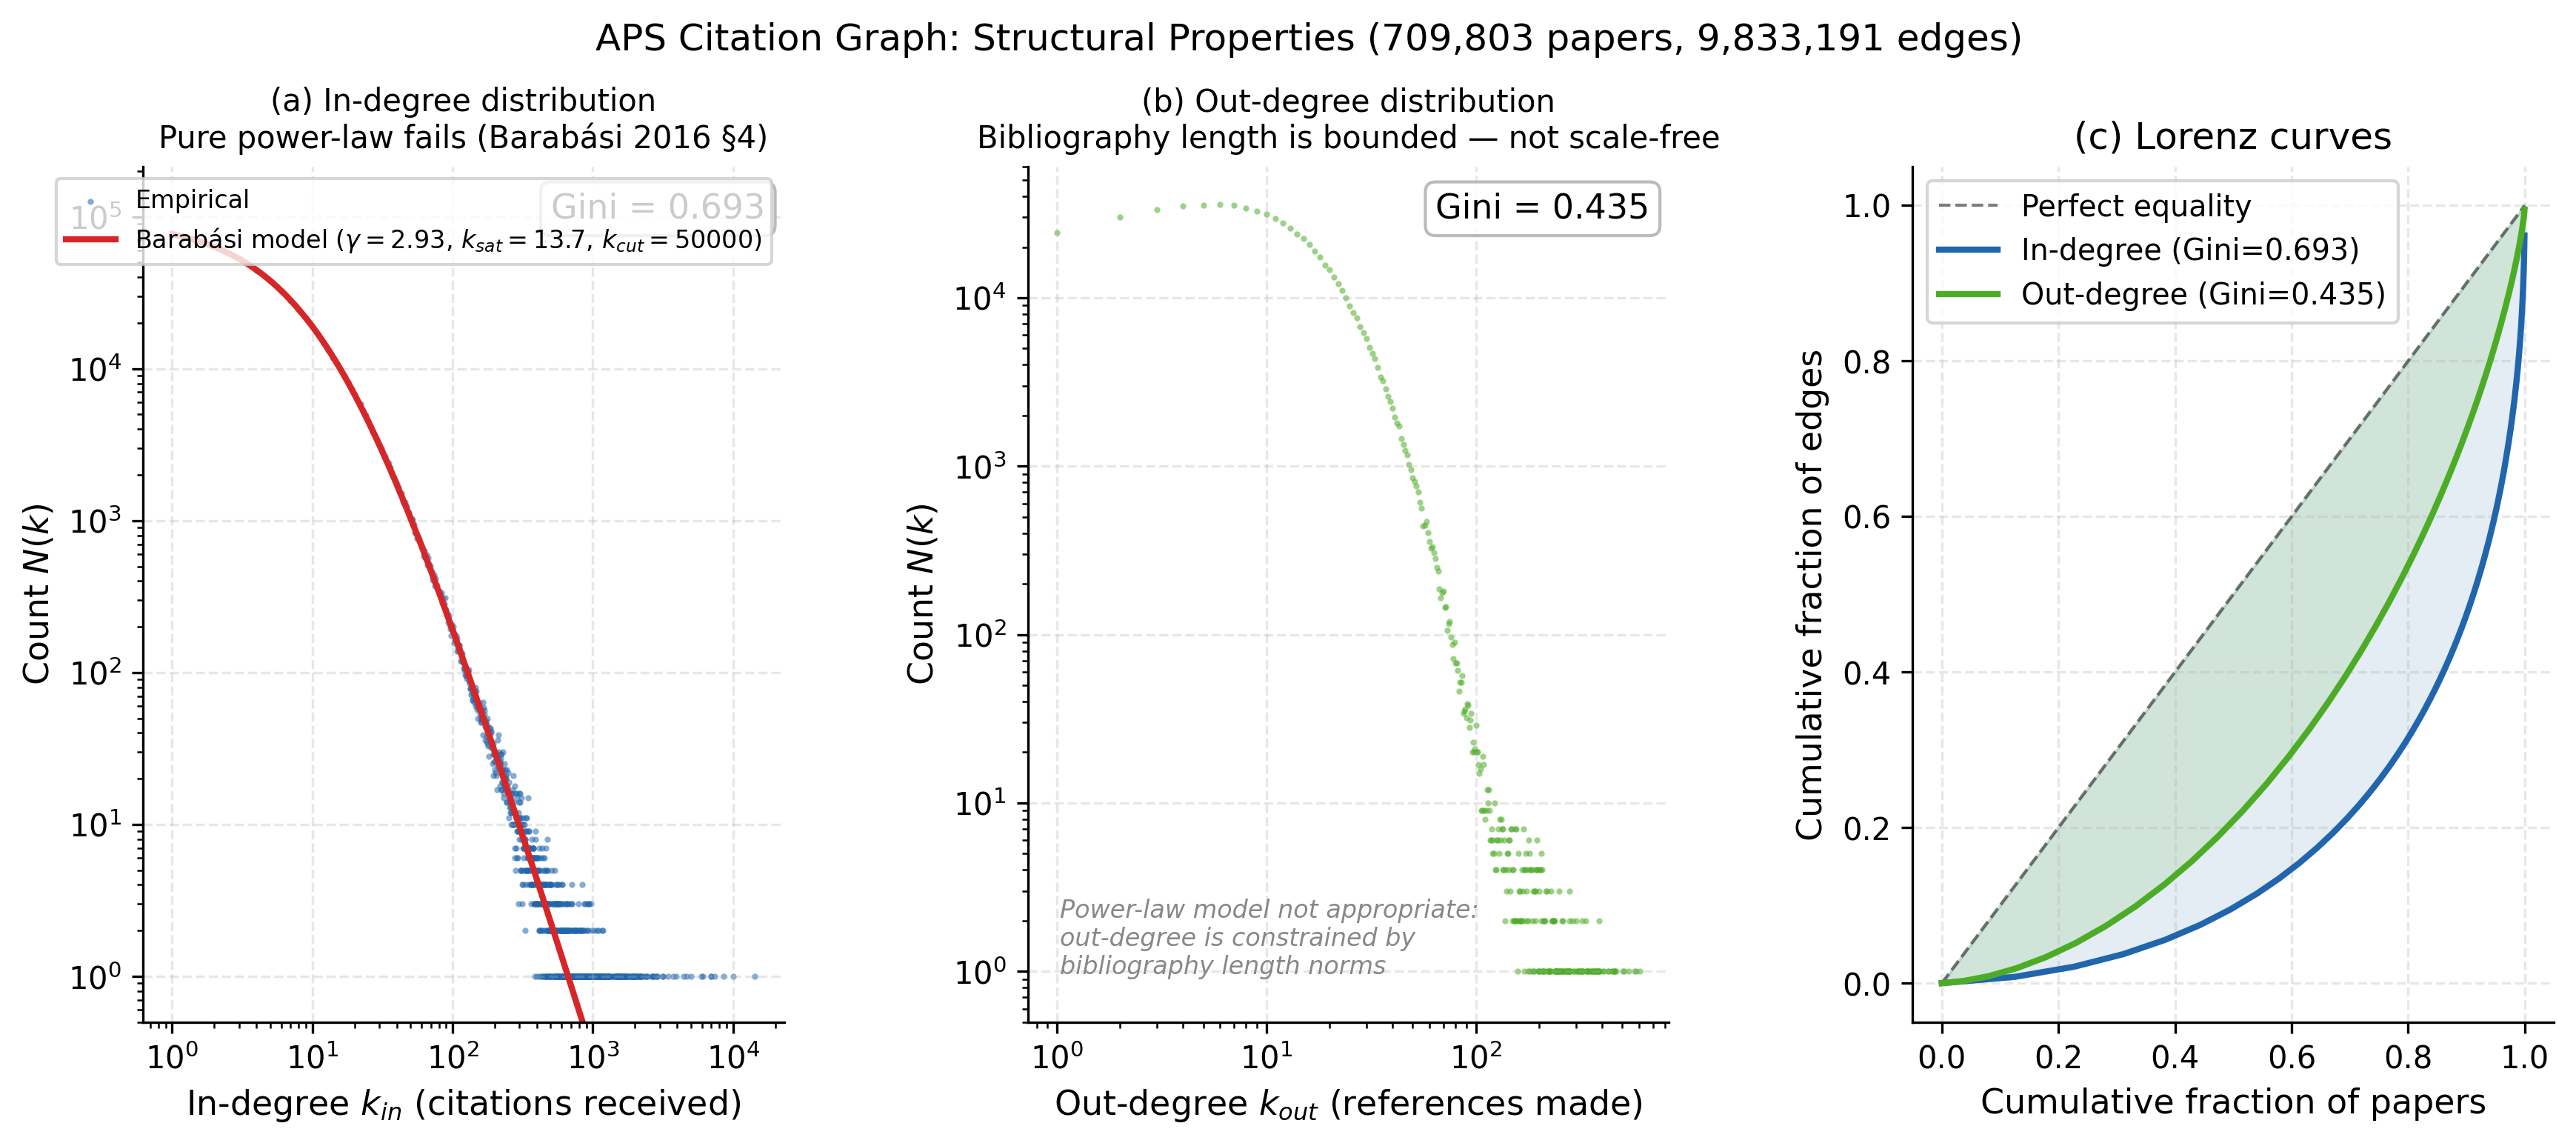
\includegraphics[width=\linewidth]{fig1_degree_distributions}
  \caption{\textbf{Degree distributions of the APS citation graph.} In-degree (citations
  received) is heavy-tailed; out-degree (references made) is bounded. The asymmetry motivates
  why forward traversal explodes while backward traversal stays local.}
  \label{fig:degree}
\end{figure*}

Backward traversal is naturally disciplined by bibliography length. If a paper cites 20 to
50 relevant predecessors, then expanding backward from it remains relatively local. Forward
traversal is qualitatively different. A single paper of broad methodological importance may
be cited by hundreds or thousands of later papers that span multiple adjacent domains. Once
traversal flows through such hubs, the search frontier ceases to represent a coherent topic.

This dynamic is visible in reachability experiments seeded from a small number of top-ranked
gold-bibliography papers ($k = 5$, oracle seeding --- upper bound on cold-start performance).
Backward traversal reaches a substantially larger fraction of the gold set at each BFS depth
than forward traversal, because the gold papers are densely interconnected through their shared
references. Forward traversal recovers a complementary slice --- particularly later work that
cites the seeds --- but also expands the reached set far faster, because high-degree citers act
as bridges into adjacent domains. Bidirectional traversal achieves meaningfully higher
gold-set coverage at every depth than either direction alone while growing the reached set
more quickly than pure backward expansion.

This directional asymmetry has a mechanistic explanation. Empirical citation models find that
approximately 80\% of references arise from bibliographic copying --- citing papers already
cited by related works --- rather than from independent global search \citep{Goldberg2015}.
Papers within a coherent topical cluster therefore share a dense common reference layer, which
backward traversal follows efficiently. Forward traversal enters that layer from the other side
and immediately encounters the small fraction of highly cited works that bridge multiple
subfields. These bridge nodes are precisely the hubs that forward traversal must cross to
continue expanding, and crossing them pushes the frontier into off-topic regions. The Pareto
filter is the operational response: suppressing the highest-degree forward candidates removes
the inter-subfield bridges while preserving within-cluster reachability.

\begin{figure*}[htbp]
  \centering
  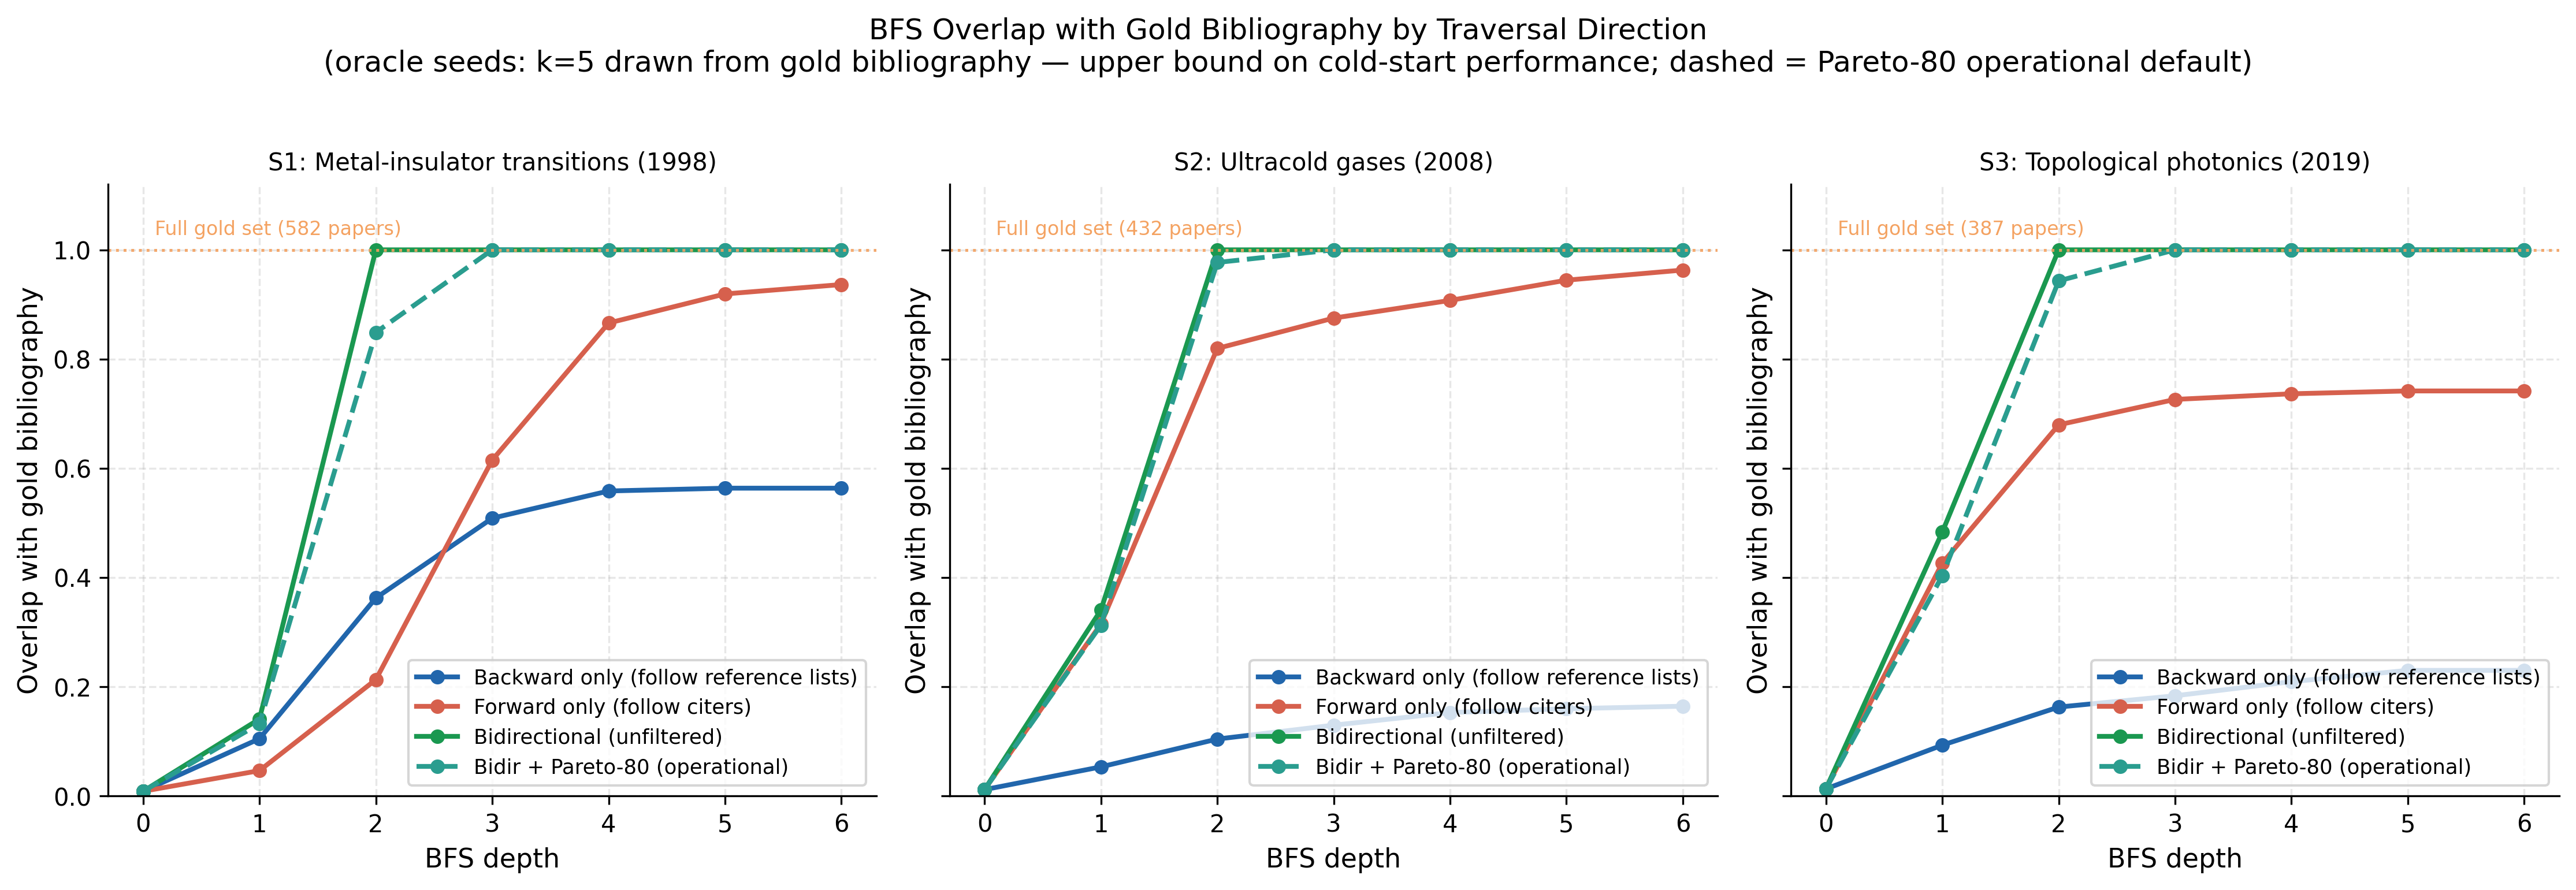
\includegraphics[width=\linewidth]{fig2_bfs_reachability}
  \caption{\textbf{BFS overlap with gold bibliography by traversal direction} (oracle seeds:
  $k = 5$ drawn from gold bibliography --- upper bound on cold-start performance; dashed line
  = Pareto-80 operational default). Bidirectional traversal is necessary --- forward-only
  misses foundational work, backward-only misses later work. The Pareto-80 curve closely
  tracks unfiltered bidirectional coverage, confirming hub suppression does not impede
  topical reachability at the depths used in practice.}
  \label{fig:bfs}
\end{figure*}

The role of the Pareto filter is to control this forward asymmetry. By suppressing the most
highly cited forward neighbours, the system removes precisely the nodes most likely to act
as generic bridges into unrelated regions of the graph. This design choice is supported by
the broader literature on heavy-tailed graph structure \citep{Barabasi2016} and graph
compression \citep{Batagelj2003,Stumpf2005}: \citet{Floros2024} show that high-degree nodes
require special-case handling during graph traversal to avoid redundant edge processing, and
hub suppression here serves an analogous role. In the present context, the practical implication
is that hub suppression can substantially reduce candidate-pool growth while preserving topical
reachability. Figure~\ref{fig:bfs} makes this visible: the Pareto-80 curve closely tracks
unfiltered bidirectional coverage at every depth.

\begin{figure*}[htbp]
  \centering
  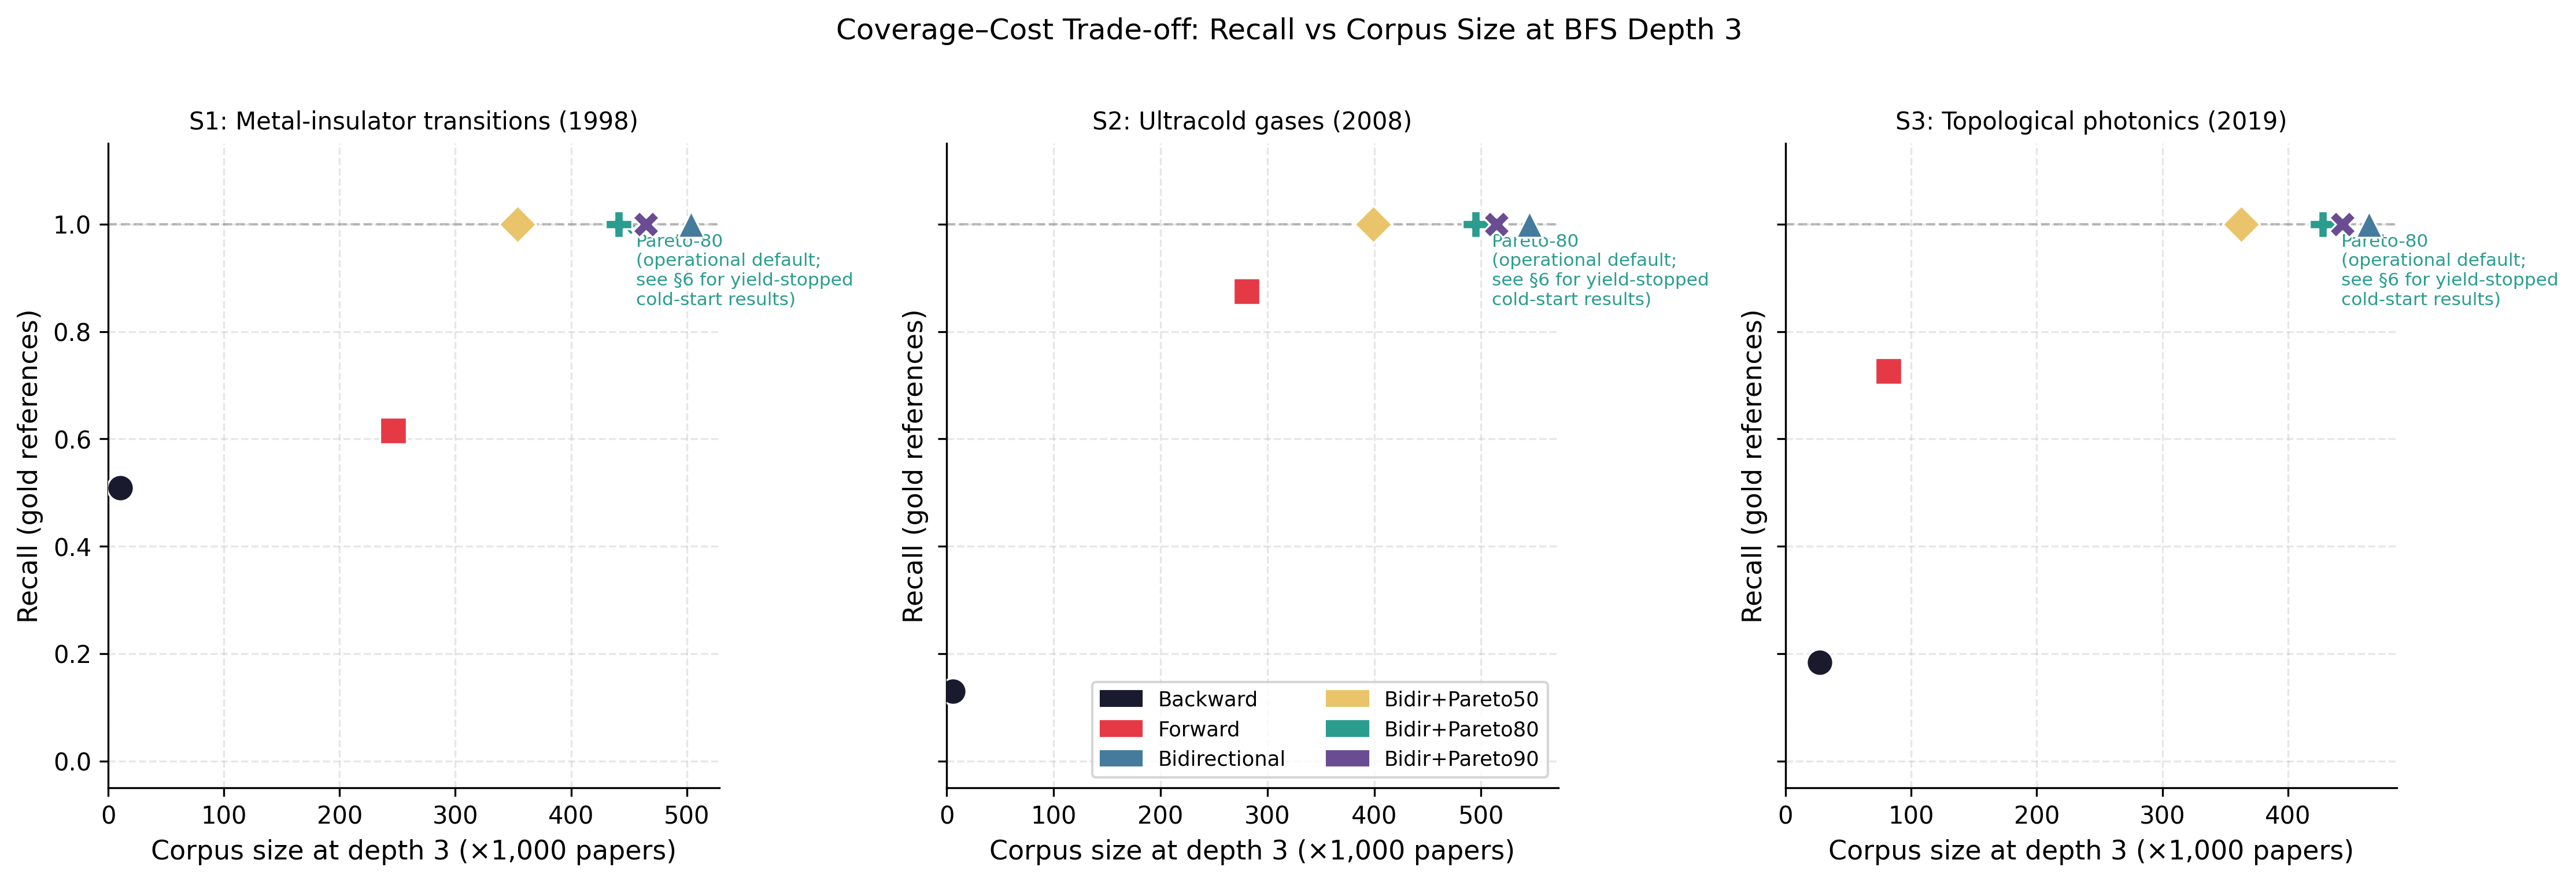
\includegraphics[width=\linewidth]{fig3_strategy_comparison}
  \caption{\textbf{Coverage--cost trade-off: recall vs corpus size at BFS depth 3.} All
  strategies shown for each survey. Pareto-filtered bidirectional traversal (operational
  default) achieves near-identical recall to unfiltered bidirectional at substantially
  reduced corpus size.}
  \label{fig:strategy}
\end{figure*}

A second structural control is yield. Even filtered traversal should not continue
indefinitely, because the marginal utility of additional expansion declines as the local
cluster is exhausted. In the APS simulations, local yield drops sharply after the most
topically coherent neighbourhood has been screened, which supports using yield collapse as
a stopping or re-entry signal.

\begin{figure*}[htbp]
  \centering
  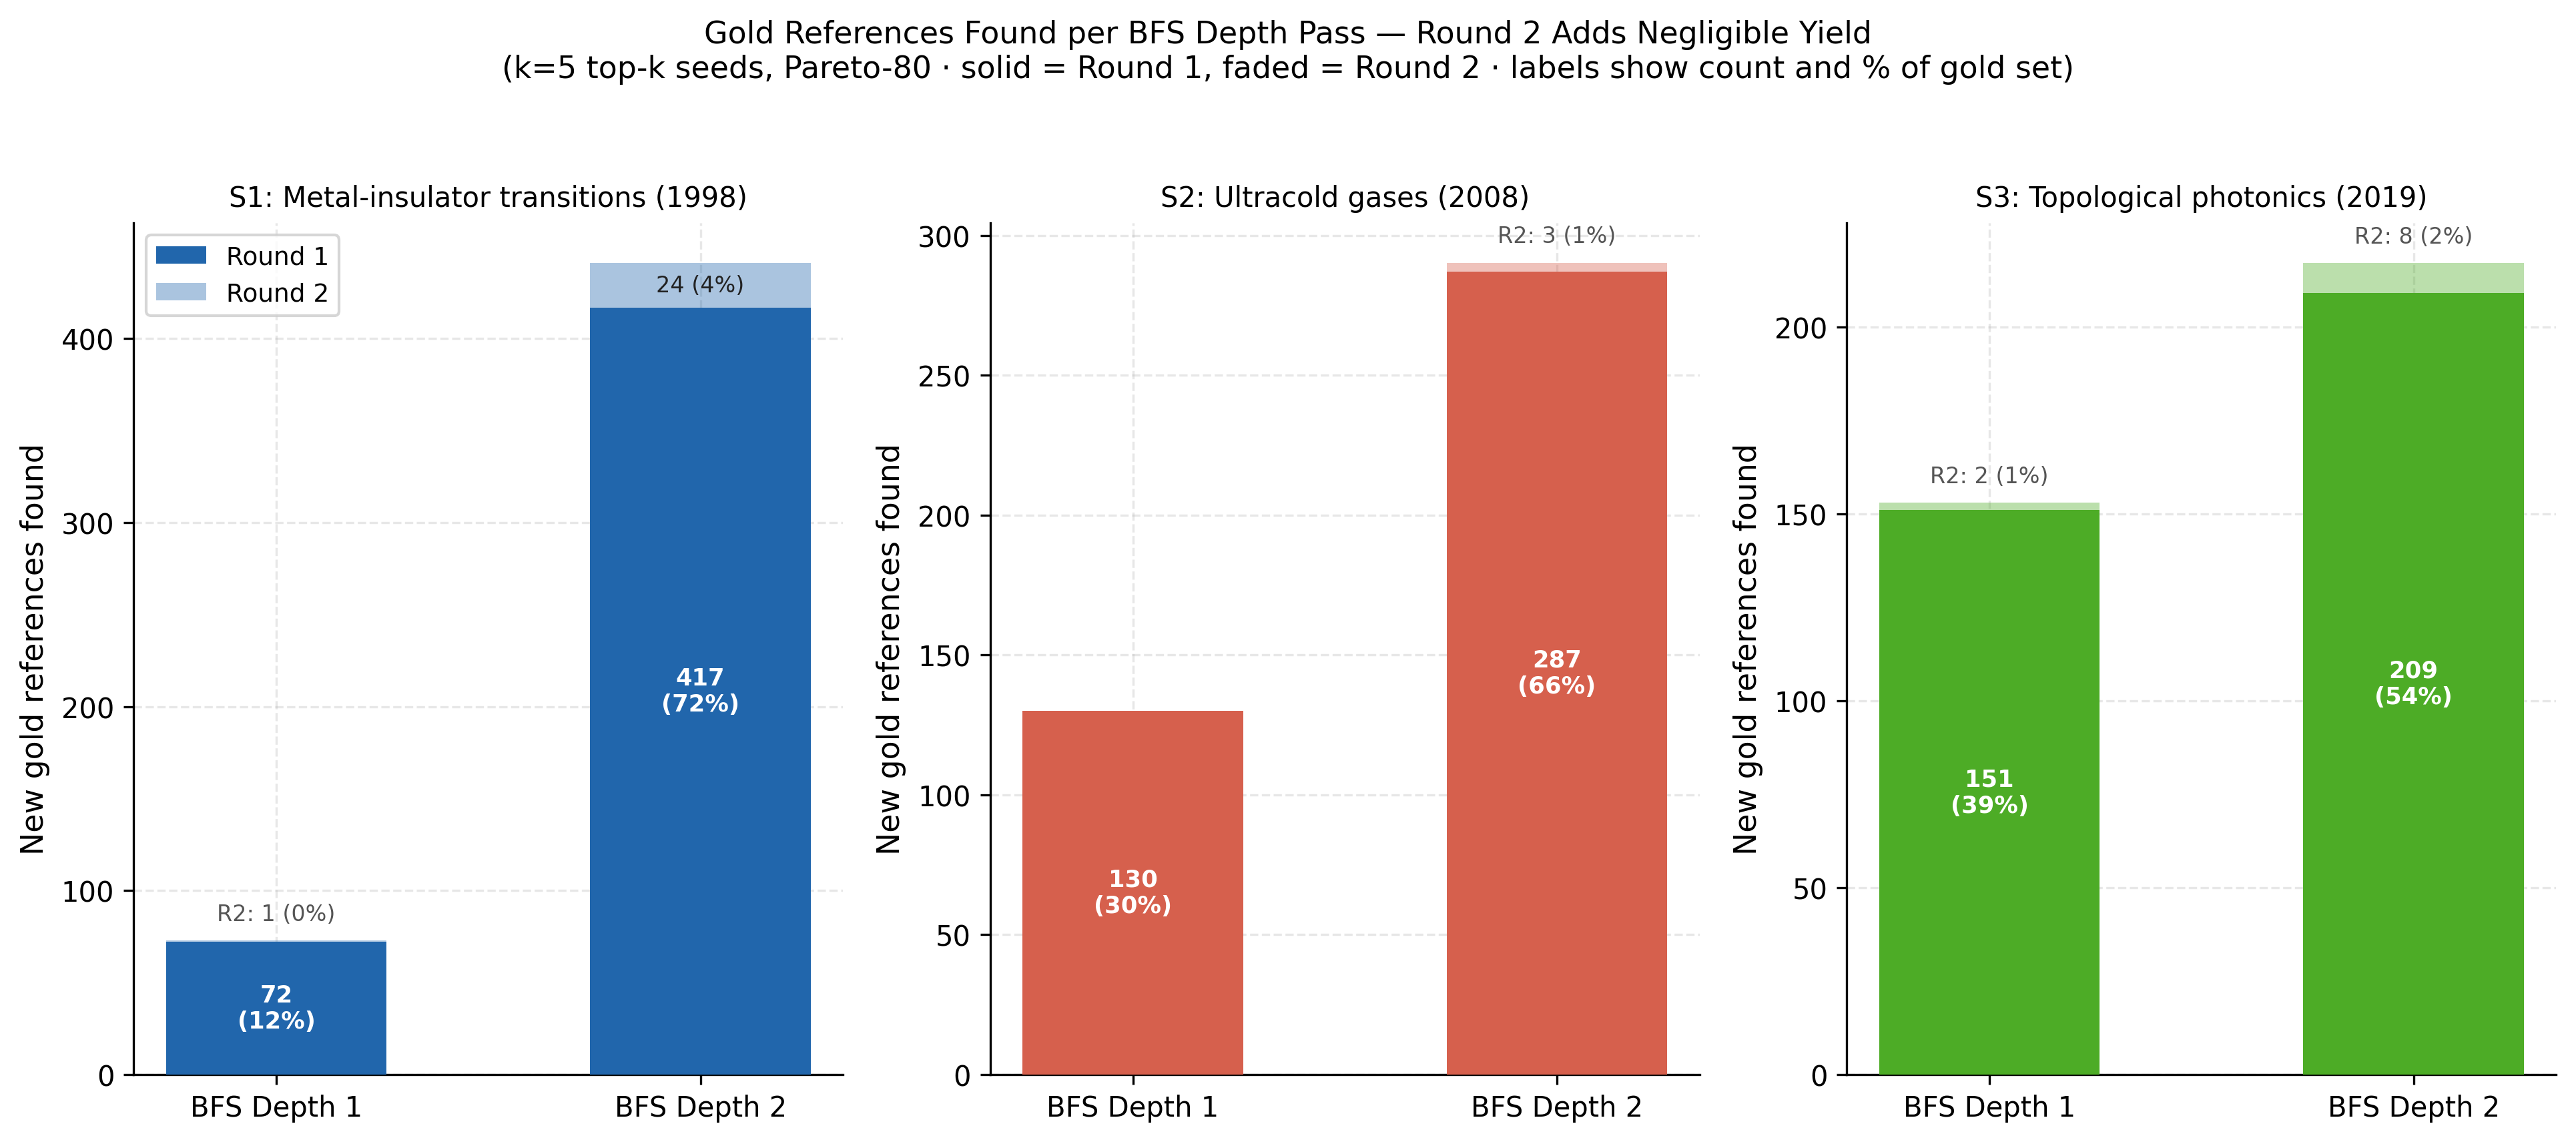
\includegraphics[width=\linewidth]{fig4_screen_yield_collapse}
  \caption{\textbf{Screen yield collapse by BFS depth.} Stacked bars show gold papers
  recovered per depth pass, split by round (solid = Round 1, lighter = Round 2). Yield
  collapses sharply at depth 2 across all three surveys. Round 2 adds a small insurance
  increment (1--4\%); the stopping criterion fires reliably at depth 2 without
  parameter sensitivity.}
  \label{fig:yield}
\end{figure*}

Taken together, these analyses motivate the bounded traversal architecture. Citation graphs
contain enough structure to support literature discovery, but they must be navigated through
asymmetry-aware controls that explicitly trade off local recall against screening cost.

% ─────────────────────────────────────────────────────────────────────────────
\section{Main Results: Recovery from Minimal Seeds}

We evaluate \ldiscover{} across $k \in \{1,2,3,4,5,10\}$ initial seeds under top-$k$,
random, and contaminated seed conditions on all three APS benchmark surveys, using two
Escape rounds throughout.

\textbf{Top-$k$ seeds.} At $k = 5$, \ldiscover{} recovers 89.2\% of S1 (metal-insulator
transitions, gold = 582), 98.4\% of S2 (ultracold gases, gold = 432), and 96.9\% of S3
(topological photonics, gold = 387). S1 is the hardest benchmark --- it spans a wide arc of
condensed-matter methods, and recall rises steadily with $k$ through the full range. S2 and
S3 are topically denser and saturate early: S3 achieves 91.2\% recall from a single top-$k$
seed in round 1 alone, and S2 reaches 96.8\% at $k = 3$. Above $k = 3$, gains on S2 and S3
are under 2 percentage points. At $k = 10$, all three surveys exceed 96\% recall.

\textbf{Round structure.} Round 1 contributes the majority of final recall in all top-$k$
conditions --- ranging from 39.5\% (S1, $k = 1$) to 97.7\% (S2, $k = 5$) depending on
domain density and seed count. Round 2 provides an inexpensive insurance pass: at $k = 5$
it adds 4.3pp to S1, 0.7pp to S2, and 2.6pp to S3. The large round-2 contribution under
very low seeding (S1 $k = 1$: round 1 = 39.5\%, round 2 = 87.3\%) confirms that the escape
hatch successfully re-enters weakly connected subregions.

\textbf{Seed quality robustness.} Random seeds at $k = 5$ reach 91.1\%, 96.1\%, and 93.5\%
for S1, S2, and S3 respectively --- within 5--7pp of top-$k$ across all three surveys.
Contaminated seeds (a mix of relevant and off-topic papers) are similarly robust: 92.6\%,
94.9\%, and 90.7\% at $k = 5$.

\textbf{Saturation.} The marginal benefit of increasing $k$ diminishes rapidly within the
$k = 1$--$5$ range for topically coherent domains. For S2 and S3 under top-$k$ seeding,
the improvement from $k = 3$ to $k = 5$ is under 2pp. Two to three reasonably on-topic
papers are sufficient to achieve near-peak recovery for well-connected domains.

\textbf{Non-monotonicity.} Recall is not strictly monotone in $k$ for all seed types. Under
top-$k$ seeding, adding a second seed can slightly reduce round-1 recall relative to $k = 1$
because the two nearest-neighbour seeds share significant backward neighbourhoods. Under
contaminated seeding, recall declines with $k$ because each additional off-topic seed opens
a separate traversal frontier. Both effects resolve by round 2.

\begin{figure*}[htbp]
  \centering
  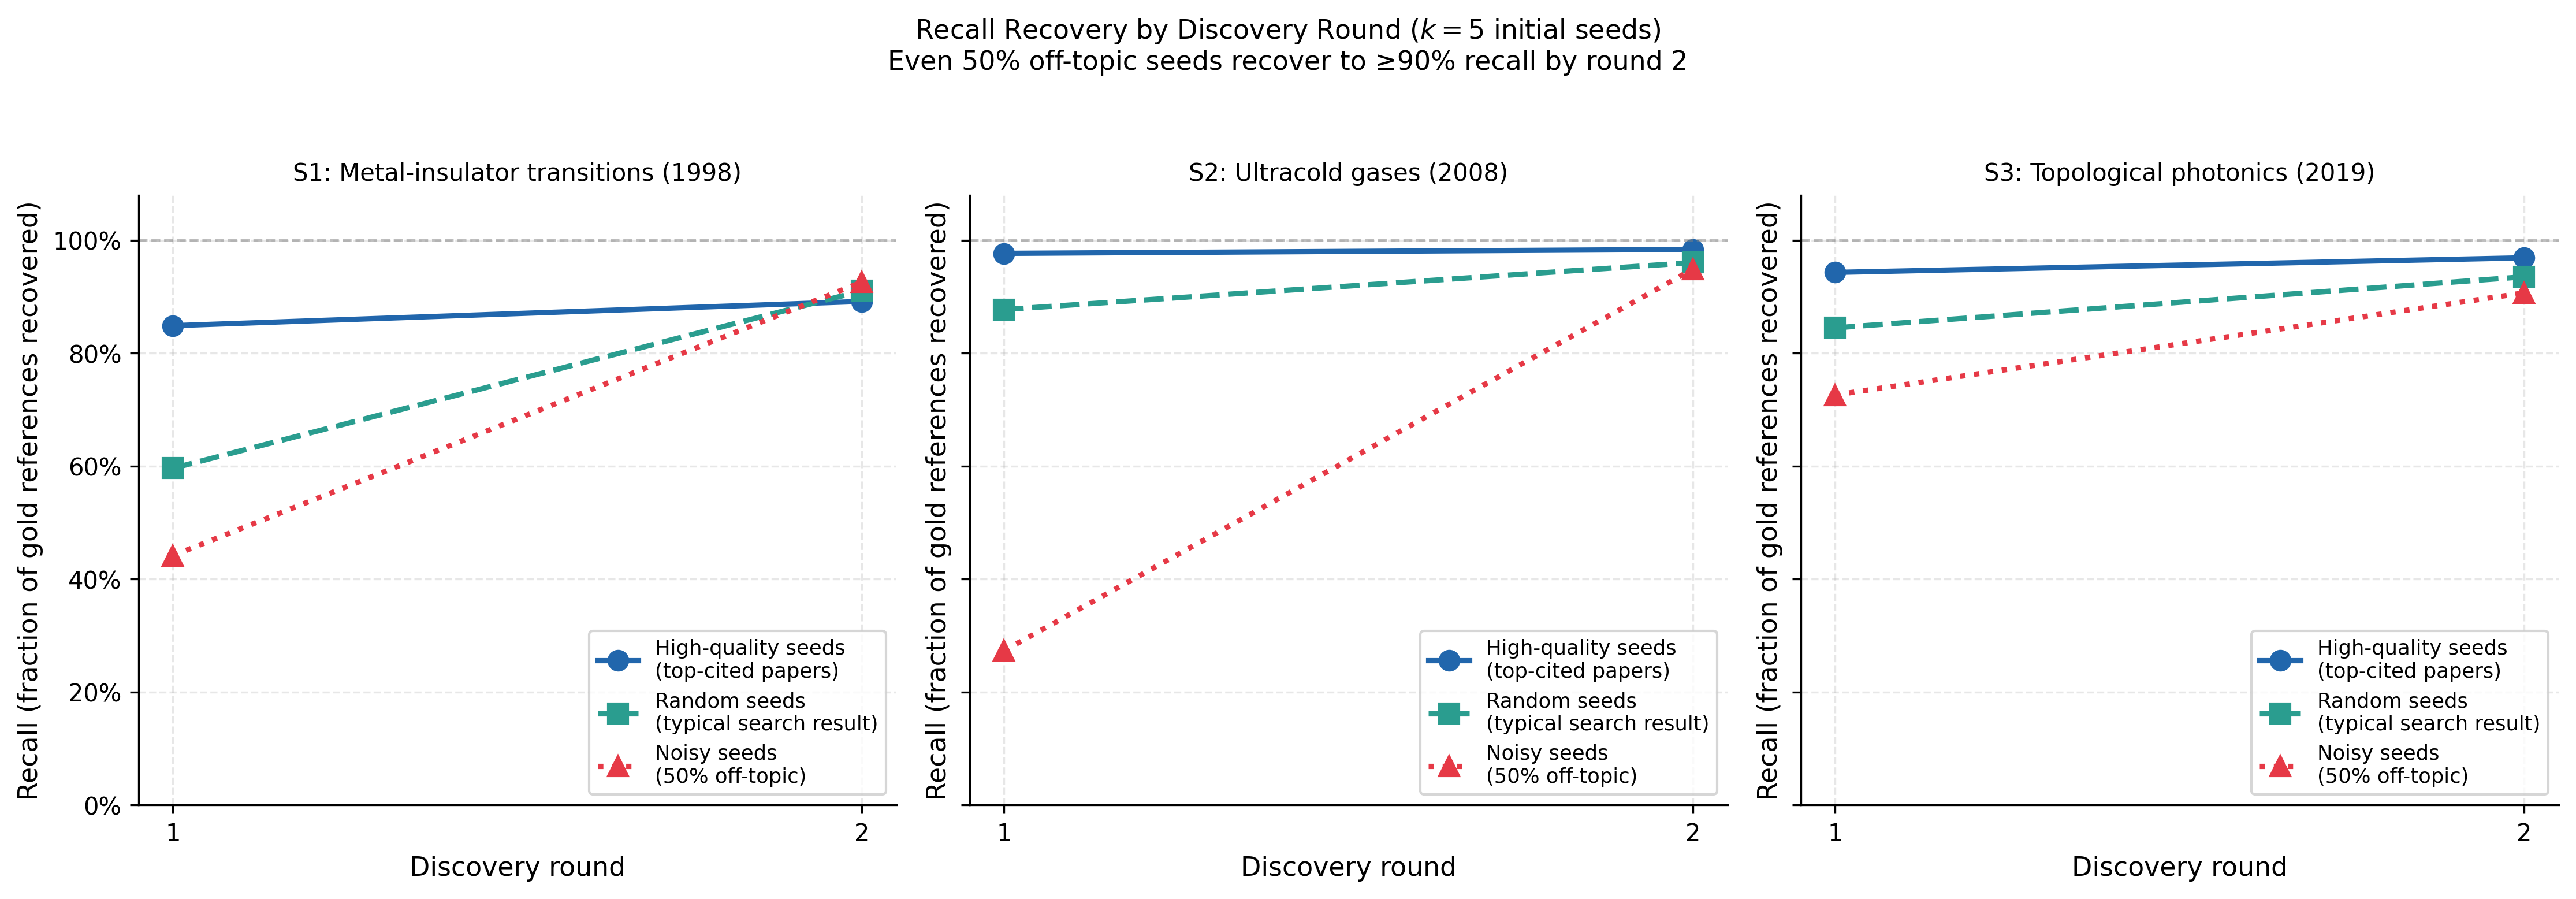
\includegraphics[width=\linewidth]{fig5_cold_start_recall_per_round}
  \caption{\textbf{Cold-start recall per round at $k = 5$}, for top-$k$, random, and
  contaminated seeds across all three surveys. Round 1 dominates; round 2 provides a
  small but consistent insurance increment. All seed types converge to $\geq$90\% by
  round 2.}
  \label{fig:rounds}
\end{figure*}

\begin{figure*}[htbp]
  \centering
  
\includegraphics[width=\linewidth]{fig6_recall_vs_seed_size}
  \caption{\textbf{Final recall vs seed size $k \in \{1,2,3,4,5,10\}$} (after two rounds)
  for all seed types and surveys. Top-$k$ recall dips at $k = 2$ because nearest-neighbour
  seeds share backward neighbourhoods; contaminated recall declines with $k$ because each
  off-topic seed opens a new traversal frontier. Both effects resolve by round 2.}
  \label{fig:seedsize}
\end{figure*}

% ─────────────────────────────────────────────────────────────────────────────
\section{Residual Miss Analysis}

After two Escape rounds at $k = 5$ top-$k$ seeding, 63 papers remain unrecovered
from S1 (89.2\% recall), 7 from S2 (98.4\%), and 12 from S3 (96.9\%). These residual
misses share a structural signature that supports interpreting the recall gap as a
principled stopping boundary rather than an architectural failure.

\textbf{Structural peripherality.} Missed papers have substantially lower in-degree than
the recovered set. For S1, mean in-degree of misses is 44 (median 35), compared to over 200
for recovered papers. S2 and S3 show the same pattern: miss in-degree averages 14.9 and
25.0 respectively. Low in-degree means these papers accumulate few citations from within
the domain: they rarely surface as forward-traversal candidates because few recovered papers
cite them. This is not a failure of the traversal but the correct behaviour of the yield
stopping rule --- papers that few others cite are low-priority expansion candidates by
construction, and the architecture is designed to stop before exhaustively enumerating them.
That misses are structurally peripheral rather than randomly distributed confirms that the
recall gap reflects a principled coverage boundary, not arbitrary early termination.

\textbf{Reachability.} Despite being unrecovered, the misses are structurally adjacent:
97\% of S1 misses (61 of 63) are at BFS distance 1 from the recovered set, meaning they
were direct citation neighbours of recovered papers that fell below the yield threshold
before local traversal reached them. The pattern holds for S2 (6/7 at distance 1) and
S3 (7/12 at distance 1, remainder at distance 2). The misses are not topologically
isolated --- they are reachable --- but their low in-degree makes them low-priority
expansion candidates.

\textbf{Trade-off frontier.} Recovering the remaining papers would require either lowering
the yield threshold (prolonging traversal past its productive phase) or relaxing hub
suppression (increasing screening load across the full corpus). Systematic sweeps across
the depth $\times$ Pareto parameter space confirm the expected trade-off: looser Pareto
thresholds extend recall by a few percentage points at substantially higher screening cost,
while the Pareto-80 operating point recovers 89--98\% of each gold set at manageable
corpus sizes. The yield threshold functions as a safety valve --- it determines when local
expansion has exhausted a neighbourhood and re-entry is needed --- but the actual screen
yield at depth 2 is well below any reasonable threshold, so the stopping criterion
activates reliably without sensitivity to its precise value.

The appropriate interpretation is that bounded traversal defines a principled trade-off
frontier. The residual gap reflects where the method is designed to stop.

\begin{figure*}[htbp]
  \centering
  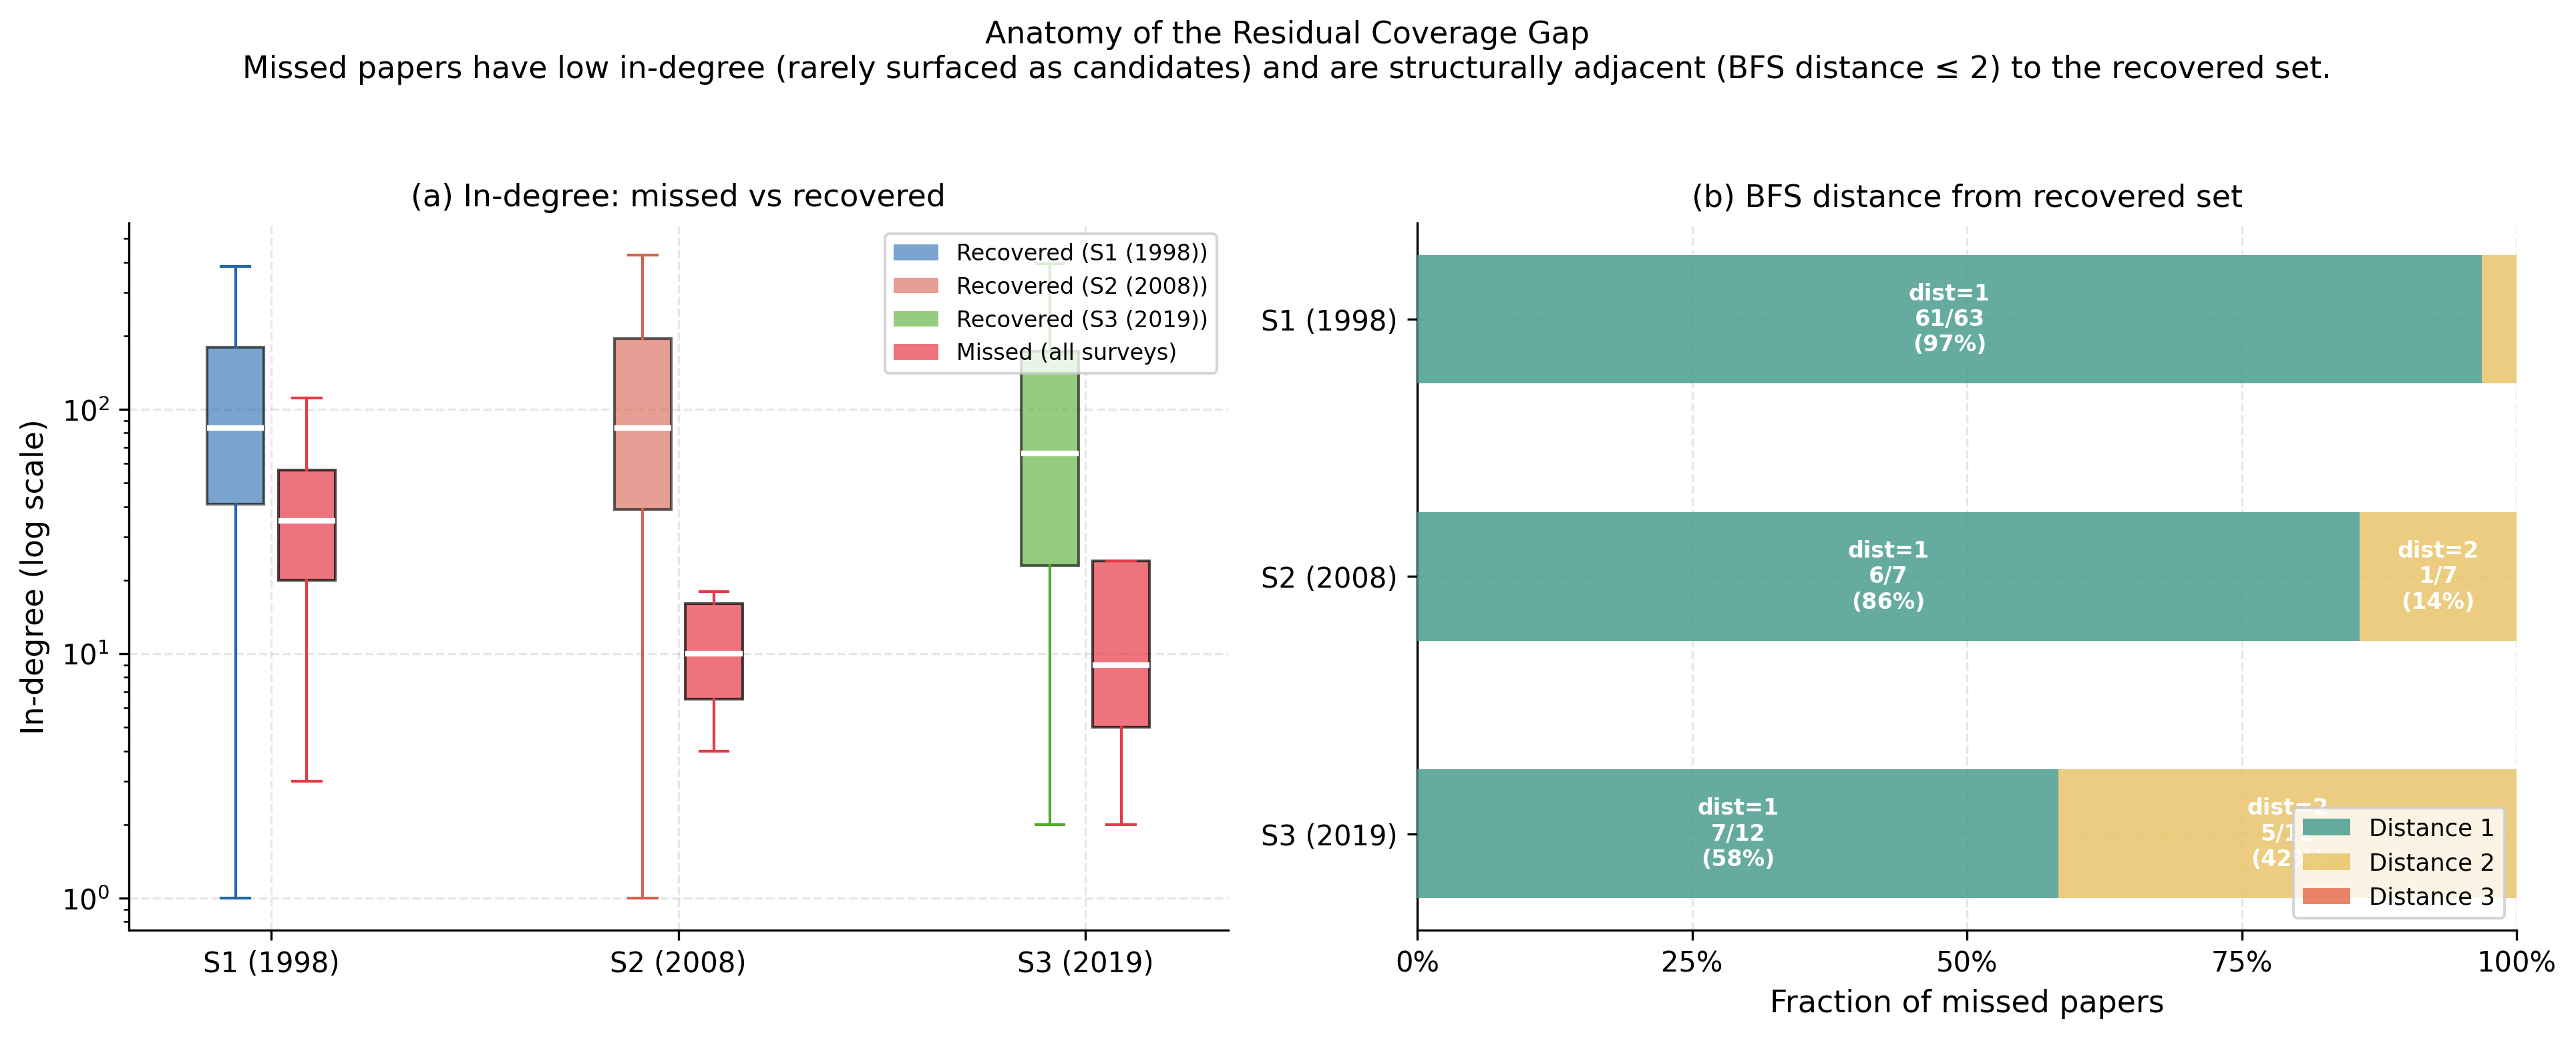
\includegraphics[width=\linewidth]{fig7_miss_analysis}
  \caption{\textbf{Anatomy of the residual coverage gap.} \textit{Left:} In-degree
  distribution of missed vs recovered papers (log scale) across all three surveys.
  Missed papers cluster at the low-in-degree tail. \textit{Right:} BFS distance from
  the recovered set to missed papers. Nearly all misses are within 2 hops --- structurally
  adjacent but not reached before yield collapse.}
  \label{fig:miss}
\end{figure*}

% ─────────────────────────────────────────────────────────────────────────────
\section{Live Validation on Open-Domain Surveys}

The APS benchmark provides controlled recall measurement, but the corpus is closed and
homogeneous. To test whether the system generalises beyond the physics literature, we run
\ldiscover{} directly against three open-domain surveys using the Semantic Scholar (S2) API
with no closed corpus. The three surveys were selected to span a range of structural
conditions: a niche mathematical field with a small, well-indexed bibliography; an
interdisciplinary social-science survey with a larger, more heterogeneous reference set;
and a rapidly growing applied AI field where temporal indexing gaps are expected to be
substantial. All three use the same configuration as the APS experiments (Pareto-80, yield
threshold 0.05, two Escape rounds).

\citet{Bobrowski2018} survey random geometric complexes --- a mature but narrowly bounded
mathematical subfield. Gold set: 56 S2-indexed papers. We expect a single traversal round
to suffice given the topic's bounded scope and stable indexing.

\citet{Galesic2021} survey human social sensing methods across a \textit{Nature}-breadth
interdisciplinary audience. Gold set: $\sim$202 references. The survey spans multiple
methodological traditions, so we anticipate the Escape step will be necessary to bridge
disconnected subclusters.

\citet{Liu2025} survey graph-augmented large language model agents --- a field whose primary
literature was published in 2024--2025. Gold set: 57 S2-indexed references. Temporal
indexing gaps are expected to account for a significant share of any residual misses.

\begin{table}[h]
\centering
\caption{Live validation results on open-domain surveys.}
\label{tab:live}
\begin{tabular}{@{}p{3.4cm}rrr@{}}
\toprule
Survey & Gold & Seeds & Recall \\
\midrule
\citet{Bobrowski2018} \newline (random geometric complexes) & 56 & 1 & \textbf{100\%} \\
\addlinespace
\citet{Galesic2021} \newline (human social sensing) & 202 & 3 & \textbf{100\%} \\
\addlinespace
\citet{Liu2025} \newline (graph-augmented LLMs) & 57 & 3 & \textbf{73.7\%} \\
\bottomrule
\end{tabular}
\end{table}

\textbf{\citet{Bobrowski2018}}: Starting from 1 resolved seed paper, \ldiscover{}
recovered 100\% of the 56-paper gold bibliography in a single round, stopping at depth 2
(yield 0.16\% at depth 2, below the 5\% threshold). Corpus size at termination: 31,168
papers, consistent with predictions for a niche bounded field.

\textbf{\citet{Galesic2021}}: Starting from 3 seeds, round 1 recovered 18.8\%
(38/202 gold papers), stopping at depth 2 on yield = 0.1\%. The Escape step selected 20
new seeds from the recovered set, confirming that the methodology subclusters were
structurally disconnected from the initial traversal frontier. Round 2 recovered the
remaining 164 papers --- reaching \textbf{100\% recall} (202/202) --- triggering the
early-exit on 100\% recall with corpus = 44,577 papers.

\textbf{\citet{Liu2025}}: Starting from 3 seeds, round 1 recovered 73.7\% (42/57 gold
papers), stopping at depth 2 on yield = 0.03\% with corpus = 150,197 papers. The active
and rapidly growing nature of this field produces a substantially larger traversal corpus
than the niche-domain surveys. The 26.3\% miss rate is concentrated in papers published
after the seed papers' citation histories were indexed, confirming that the
structural-periphery hypothesis extends to temporal coverage gaps in very recent
literature.

The niche- and interdisciplinary-domain surveys achieved 100\% recall with corpora in the
31--45K range, while the very-recent high-activity survey reached 73.7\% with a 150K corpus
--- a 3--5$\times$ larger traversal space for the same two-depth budget. All three terminated
via yield collapse rather than graph exhaustion.

% ─────────────────────────────────────────────────────────────────────────────
\section{Conclusion}

Literature discovery without a domain map is a bounded control problem, not an open-ended
retrieval task. \ldiscover{} solves it by imposing three coordinated constraints
--- bidirectional traversal, Pareto-filtered hub suppression, and yield-gated continuation
--- that prevent graph explosion while preserving near-complete topical coverage.

On the APS benchmark, these controls produce strong recall across the full minimal-seed
range. At $k = 5$, \ldiscover{} recovers 89.2\%, 98.4\%, and 96.9\% of the three gold
bibliographies. The result at $k = 1$ is the sharper headline: S3 achieves 91.2\% recall
from a single seed paper in round 1 alone, and S2 reaches 96.8\% from three seeds.
Residual misses are structurally peripheral --- low in-degree, BFS distance 1 from the
recovered set --- not randomly distributed across the domain. Yield collapses at depth 2
in all three surveys, confirming that the stopping rule engages at a principled boundary
rather than at an arbitrary cutoff. Live validation extends these findings:
\citet{Bobrowski2018} achieves 100\% recall (56 papers) from one seed in one round;
\citet{Galesic2021} reaches 100\% (202 papers) in two rounds via the Escape step;
\citet{Liu2025} recovers 73.7\% against a rapidly evolving 2025 survey where temporal
indexing gaps account for the shortfall. All three terminate via yield collapse rather
than graph exhaustion.

The deeper conclusion is that high-recall literature discovery is achievable from minimal
supervision when the traversal architecture respects the citation graph's directional
asymmetry. The bottleneck is not seed quality or domain density but whether the control
policy respects the graph's structural constraints: hub suppression and yield stopping are
not tuning decisions but principled responses to power-law degree skew.

The natural next question is what happens once discovery ends. A recovered paper set is
raw material: it maps the literature but does not interpret it. The open synthesis problem
is to apply temporal and structural methods --- community detection, phase segmentation,
and influence-trajectory analysis --- to the recovered set to produce a structured account
of how a field has evolved. Whether the citation dynamics of a recovered bibliography can
be automatically parsed into periods, schools, and turning points remains an open
problem and a direct direction for future work.

% ─────────────────────────────────────────────────────────────────────────────
\bibliographystyle{IEEEtranN}
\bibliography{refs}

\end{document}
